\newpage

\section{Supplementary material}
Using NeuroBench to analyze the performance of the algorithms on the tasks allows us to return the histograms for all of the algorithms. These histograms show the results of all 1000 runs and show how consistently a model is able to perform its task.
\begin{figure}[h]
    \centering
    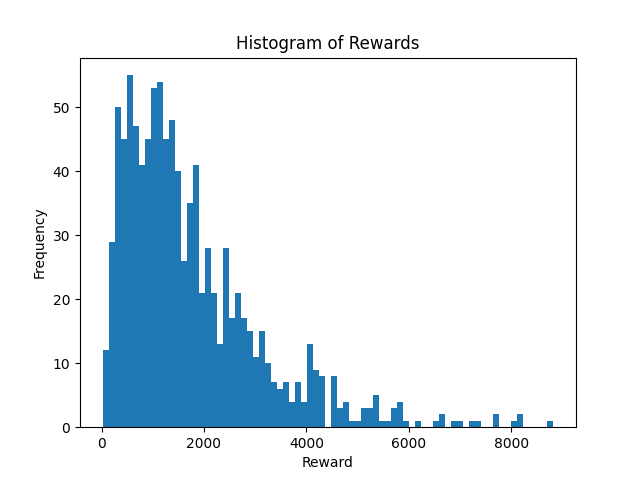
\includegraphics[width = .45\textwidth]{Figures/ANN_histogram1K.png}
    \caption{Histogram for the ANN with one hidden layer of size 246.}
    \label{fig:enter-label}
\end{figure}

\begin{figure}[h]
    \centering
    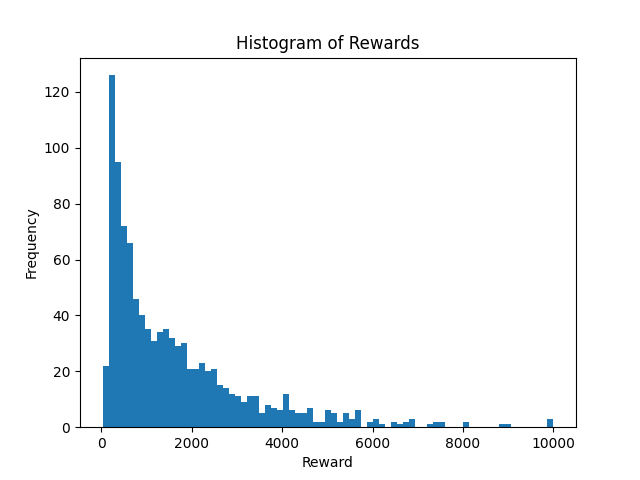
\includegraphics[width = .45\textwidth]{Figures/SNN_histogram1K_noLeak.png}
    \caption{Histogram for the SNN with one hidden layer of size 246, no leak.}
    \label{fig:enter-label}
\end{figure}

\begin{figure}[h]
    \centering
    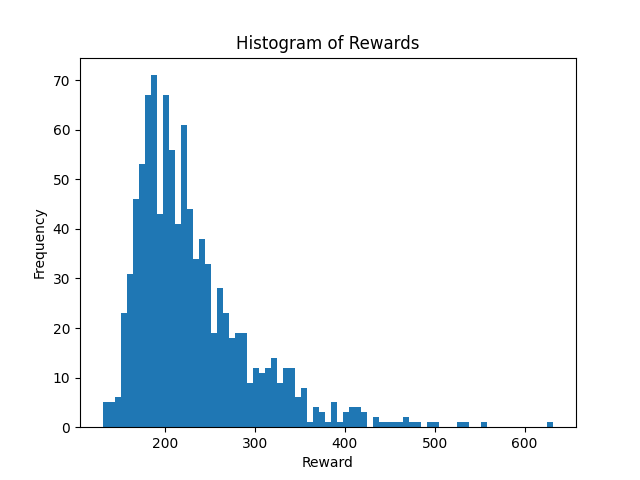
\includegraphics[width = .45\textwidth]{Figures/SNN_histogram1K_higher_leaks.png}
    \caption{Histogram for the SNN with one hidden layer of size 246, with $\beta=0.65$}
    \label{fig:enter-label}
\end{figure}